\section{Data and Experimental Design}
\label{sec:data}

\subsection{Study Design and Evidence Map}
\label{subsec:data_sources}

The empirical analysis covers Washington, DC, New York City, and Vancouver
from 1 January 2020 through 31 December 2022. These cities were selected
because each provides geocoded incident records and a large public
bicycle-system archive over a common period. Crime records were obtained
from the Metropolitan Police Department of the District of Columbia, the
New York City Police Department, and the Vancouver Police Department open
data portals \citep{dc_crime_data,nypd_crime_data,vpd_crime_data}. Bicycle
trips were obtained from Capital Bikeshare, Citi Bike, and Mobi by Rogers,
respectively \citep{capital_bikeshare_data,citibike_data,mobi_data}.

Figure~\ref{fig:problem_chain} links the three research questions to the
corresponding evidence. RQ1 concerns a population limit and is answered analytically.
RQ2 asks whether a finite-sample entropy difference can be separated from
sparse-state bias and a design-conditioned null. RQ3 applies that
distinction to lagged bicycle mobility and crime counts. Held-out prediction
is evaluated as a consequence rather than as a substitute for those questions.

\begin{figure}[!t]
\centering
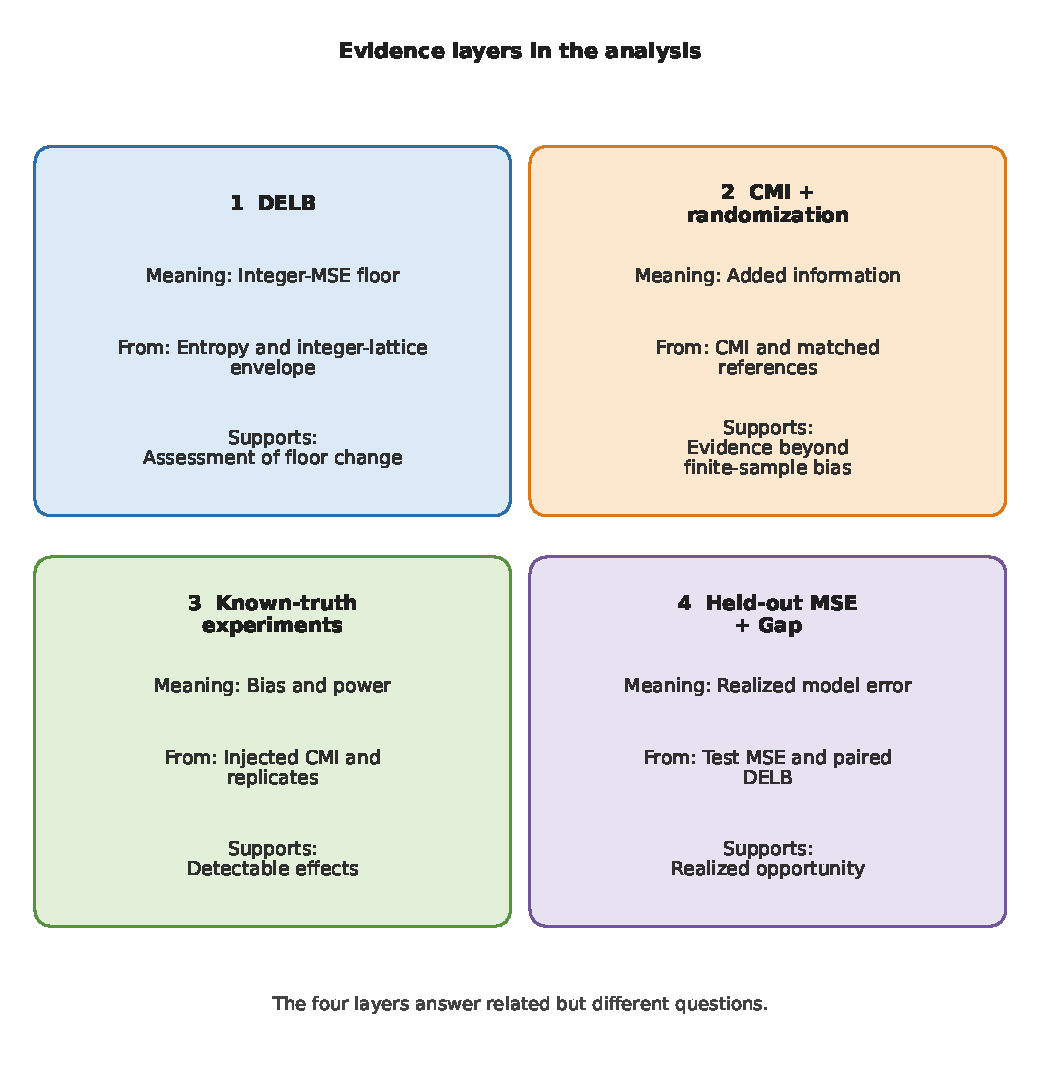
\includegraphics[width=\textwidth]{figures/problem_chain/unified_problem_chain.pdf}
\caption{Unified question-to-evidence chain. A population lower-bound
change, a calibrated finite-sample information gain, and an improvement in
realized prediction are distinct claims. CMI denotes conditional mutual
information, and DELB denotes the Discrete Entropy Lower Bound.}
\label{fig:problem_chain}
\end{figure}

Figure~\ref{fig:analysis_workflow} summarizes data processing. Crime
and bicycle records were first standardized as event-level data. They were
then aggregated to complete daily panels on a common 1~km grid. The upper
branch estimates conditional entropy, conditional mutual information (CMI),
and the DELB; the lower branch evaluates matched integer-valued
predictors. Their outputs are combined only after the information sets and
evaluation periods have been aligned.

\begin{figure}[!t]
\centering
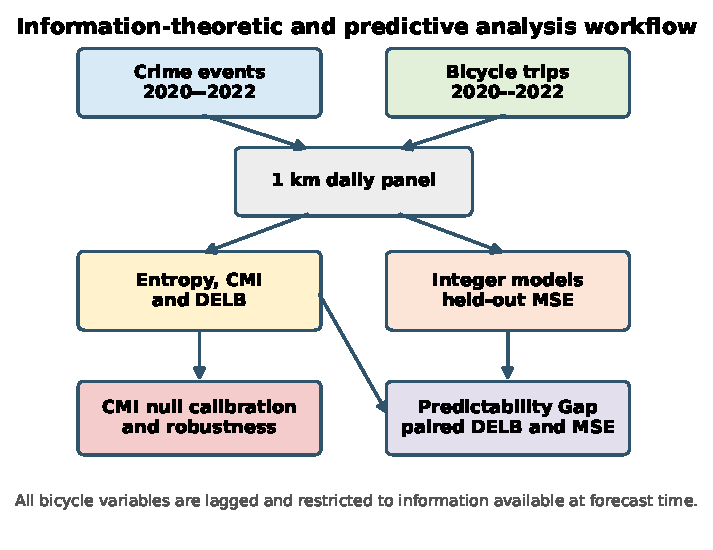
\includegraphics[width=\textwidth]{figures/e11/e11_analysis_workflow.pdf}
\caption{Data-processing and matched-analysis workflow. All
bicycle variables are lagged and restricted to information observed when
the one-day-ahead forecast is issued.}
\label{fig:analysis_workflow}
\end{figure}

\subsection{Crime Events and Cross-City Harmonization}
\label{subsec:crime_data}

The raw crime files were harmonized at the event level. We retained the
authoritative standardized field \texttt{crime\_type\_unified} and did not
reclassify it in later experiments. The analytic outcome combines three
mutually exclusive categories: property theft, vehicle theft, and burglary.
The source-category crosswalk is reported in
Appendix~\ref{app:empirical_details}. Events were assigned to their source
file's calendar year; 35 Washington, DC records whose event dates fell
outside that year were placed in a reason-coded exclusion table. Stable
event identifiers, source file hashes, source row numbers, original
categories, timestamps, and coordinates were retained for auditability.

Standardization produced 503,157 valid crime events. After applying the prespecified
spatial domain described below, \TotalCrimeEvents{} events entered the
complete analytic panels. The primary prediction target,
\(C_{c,i,t}\), is the unbinned daily count of all three harmonized
categories in city \(c\), grid cell \(i\), and local calendar day \(t\).
Category-specific counts are used only in the heterogeneity analysis.

\subsection{Bicycle Trips and Endpoint Flows}
\label{subsec:bicycle_data}

Schemas differed across the three systems and changed during the study period.
We standardized them to a common trip interface with start and end times, station identifiers,
station names, endpoint coordinates, coordinate provenance, source
identifiers, and quality-control flags. Input files were processed in
chunks, and month assignment was determined by trip start time. Blank rows
and trips assigned to a different source month were retained in
reason-coded exclusion tables. Official ride identifiers were required to
be unique after deterministic first-record retention. Exact duplicate
Vancouver records without an official unique ride identifier were retained
and flagged rather than silently removed.

Source coordinates were used when valid. Missing coordinates in Washington, DC and
New York were recovered from robust station-month medians and
temporally adjacent observations. Vancouver endpoints were matched first
to the official station identifier and then to a unique normalized station
name in the supplied official station file. Workshop, service, testing,
yard, storage, production, temporary, and valet nodes were marked
non-public. Unresolved endpoints were preserved in the standardized trip
table but were ineligible for spatial flow at that endpoint; a trip could
still contribute its other resolved public endpoint.

For each grid--day, departures and arrivals define
\(B^{\mathrm{out}}_{c,i,t}\) and \(B^{\mathrm{in}}_{c,i,t}\), with total
endpoint flow
\[
B^{\mathrm{total}}_{c,i,t}
=B^{\mathrm{out}}_{c,i,t}+B^{\mathrm{in}}_{c,i,t}.
\]
The primary mobility variable is the one-day lag of total flow. This measure captures
observable activity at both ends of a trip without including the
deterministically redundant total and net flow together with inflow and
outflow in the same entropy state. Standardization retained 87,208,600
trips; \TotalBicycleTrips{} trips had at least one flow-eligible endpoint
inside the analytic grids.

\subsection{Spatial and Temporal Panel Construction}
\label{subsec:panel_construction}

Coordinates were projected in the appropriate city coordinate reference
system and assigned to deterministic 1~km square cells anchored to the
projected coordinate-system origin. Two training-period-frozen populations
were prespecified for city-level point estimation. The complete
crime-supported domain contains every cell with at least one crime event
during 2020--2021. The bicycle-covered domain is the subset of those cells
with positive total bicycle flow during the same training period. Neither
definition uses a 2022 record. Bicycle endpoints outside the complete
crime-supported domain remained in reconciliation outputs but were not
used in either analytic population.

Every retained grid was crossed with all 1096 calendar days, including
zero-crime and zero-flow days. The resulting complete panel contains
\TotalPanelRows{} grid--day observations across 1133 cells. The
bicycle-covered panel is a fixed spatial subset of this complete panel; it
was not reconstructed from the set of nonzero-flow days. Lag construction
removed the first day of each grid only when a lagged analysis was
performed.

The temporal split was fixed before model estimation: 2020--2021 for
training, January--June 2022 for validation, and July--December 2022 for
testing. Spatial eligibility, bicycle coverage, and bicycle discretization
thresholds were determined from training records only. Model
hyperparameters were selected using training and validation data only.
The test period defined neither the domains nor any threshold, model
setting, or eligibility decision. All predictors used for a forecast were
available at issuance: no concurrent or future crime or mobility record
entered the information sets. Table~\ref{tab:variable_availability} makes
this timing explicit, and Table~\ref{tab:descriptive_statistics} summarizes
the complete panels.

\begin{table}[!htbp]
\caption{Variables, analysis units, and forecast-time availability. ``Yes,
lagged'' indicates that only information from the previous aggregation
period was used for one-period-ahead prediction.}
\label{tab:variable_availability}
\centering
\begin{tabularx}{\textwidth}{
>{\RaggedRight\arraybackslash}p{2.1cm}
>{\RaggedRight\arraybackslash}X
>{\RaggedRight\arraybackslash}p{1.7cm}
>{\RaggedRight\arraybackslash}p{1.8cm}
>{\RaggedRight\arraybackslash}p{2.0cm}}
\toprule
\textbf{Variable} & \textbf{Meaning and role} & \textbf{Spatial unit} &
\textbf{Temporal unit} & \textbf{Available at forecast time}\\
\midrule
Crime count & Daily incidents in the three harmonized crime categories;
unbinned prediction target & 1 km grid & Day & Target, no\\
Lagged crime & Previous-period crime count, discretized into four levels
(0, 1, 2, and 3+); baseline state & 1 km grid & Previous day & Yes, lagged\\
Bicycle inflow & Arrivals at resolved public endpoints; mobility primitive &
1 km grid & Previous day & Yes, lagged\\
Bicycle outflow & Departures from resolved public endpoints; mobility
primitive & 1 km grid & Previous day & Yes, lagged\\
Total bicycle flow & Sum of inflow and outflow, discretized using
training-period thresholds; added-data state & 1 km grid & Previous day &
Yes, lagged\\
Calendar state & Day of week, meteorological season, and public-holiday
status; baseline state & City/grid & Forecast day & Yes\\
Grid identifier & Fixed spatial state defined before validation and testing;
baseline state & 1 km grid & Fixed & Yes\\
\bottomrule
\end{tabularx}
\end{table}


\begin{table}[H]
\caption{Descriptive statistics for the complete 1 km grid--day panels, 2020--2022.}
\label{tab:descriptive_statistics}
\begin{adjustwidth}{-\extralength}{0cm}
\centering
\begin{tabular}{lrrrrrrr}
\toprule
\textbf{City} & \textbf{Grids} & \textbf{Grid--days} &
\textbf{Crime events} & \textbf{Bike trips} &
\textbf{Mean crime} & \textbf{Mean bike flow} & \textbf{Zero crime}\\
\midrule
Washington, DC & 186 & 203,856 & 71,397 & 7,620,562 & 0.350 & 72.95 & 77.0\%\\
New York City & 806 & 883,376 & 359,284 & 76,418,121 & 0.407 & 172.82 & 79.7\%\\
Vancouver & 141 & 154,536 & 72,447 & 2,231,293 & 0.469 & 27.37 & 75.3\%\\
\bottomrule
\end{tabular}
\end{adjustwidth}
\end{table}


Crime was sparse at the grid--day scale: zero counts represented
75.3--79.7\% of observations. New York contributed the largest system and
the highest mean daily bicycle endpoint flow, whereas Vancouver had the
highest mean property-crime count per grid--day. We report
city-specific quantities rather than treat the pooled records as exchangeable.

\subsection{Descriptive Analysis}
\label{subsec:descriptive_analysis}

Monthly and spatial summaries were computed before entropy estimation. At
the monthly level, Spearman correlations between crime and bicycle flow
were 0.505 in Washington, DC, 0.603 in New York, and 0.221 in Vancouver.
Across grids, the corresponding correlations of three-year totals were
0.637, 0.651, and 0.633. The top decile of grids accounted for 43.9, 54.3,
and 54.1\% of crime but 67.5, 89.0, and 79.7\% of bicycle flow,
respectively. These are descriptive associations and do not condition on
crime history or calendar state.

The corresponding spatial-concentration and monthly-series figures are
reported in Section S6 of the independent Supplementary Materials, so that
the main text proceeds directly to the DELB estimand and its finite-sample
validation.

\subsection{Evaluation Design Overview}
\label{sec:methods}

Analysis proceeded in the order of the research questions. We first
operationalized the target and information sets, then evaluated the
numerical DELB and examined finite-sample CMI behavior with known-truth
simulation and support diagnostics, estimated city and local point values,
calibrated them against three randomization references, and only then
compared matched held-out predictions. Fano, crime-type, and
alternative-specification analyses served as secondary checks.

\subsection{Targets and Operational Information Sets}
\label{subsec:operational_information_sets}
\label{subsec:methods_information_sets}

For the application, the generic target in Section~\ref{sec:theory} is
\begin{equation}
X_t\longmapsto C_{c,i,t}\in\mathbb Z_{\geq0},
\label{eq:crime_count_definition}
\end{equation}
the unbinned count for city \(c\), grid \(i\), and day \(t\). Bicycle
departures and arrivals are
\begin{equation}
B^{\mathrm{out}}_{c,i,t}
=\text{departures from }(c,i,t),
\qquad
B^{\mathrm{in}}_{c,i,t}
=\text{arrivals at }(c,i,t),
\label{eq:bicycle_in_out}
\end{equation}
with primitive vector
\begin{equation}
\mathbf B_{c,i,t}
=
(B^{\mathrm{out}}_{c,i,t},B^{\mathrm{in}}_{c,i,t})^\top,
\label{eq:bicycle_primitive_vector}
\end{equation}
total and net flow
\begin{align}
B^{\mathrm{total}}_{c,i,t}
&=B^{\mathrm{out}}_{c,i,t}+B^{\mathrm{in}}_{c,i,t},
\label{eq:bicycle_total_flow}\\
B^{\mathrm{net}}_{c,i,t}
&=B^{\mathrm{in}}_{c,i,t}-B^{\mathrm{out}}_{c,i,t},
\label{eq:bicycle_net_flow}
\end{align}
and lag block
\begin{equation}
\mathbf B^{(q)}_{c,i,t}
=
(\mathbf B_{c,i,t-1},\ldots,\mathbf B_{c,i,t-q}).
\label{eq:bicycle_lag_block}
\end{equation}
Total and net flow are deterministic functions of the primitive vector and
are not entered redundantly in one entropy state.

For one-day-ahead prediction, the target remained the raw nonnegative
integer count. Only conditioning variables were discretized. The previous
day's crime count was mapped to
\(\{0,1,2,\geq 3\}\). Within each city, the positive values of lagged total
bicycle flow were divided at training-period terciles; zero flow formed a
separate state. This produced four bicycle states:
\(\{\text{zero},\text{low},\text{medium},\text{high}\}\), and the fitted
cut points were reused unchanged in validation and testing.

The baseline information state was
\begin{equation}
\mathcal{S}^{0}_{c,i,t}
=\left(i,Q_C(C_{c,i,t-1}),d_t,s_t,h_t\right),
\label{eq:empirical_baseline_state}
\end{equation}
where \(d_t\), \(s_t\), and \(h_t\) denote day of week, meteorological
season, and public-holiday status. The bicycle-augmented state was
\begin{equation}
\mathcal{S}^{B}_{c,i,t}
=\left(\mathcal{S}^{0}_{c,i,t},
Q_B(B^{\mathrm{total}}_{c,i,t-1})\right).
\label{eq:empirical_bicycle_state}
\end{equation}
Only one component differs between the matched states: lagged bicycle flow.
The design excludes concurrent or future
mobility. In sigma-algebra notation,
\begin{align}
\mathcal F^0_{c,i,t}
&=\sigma(\mathcal S^0_{c,i,t}),
\label{eq:baseline_information}\\
\mathcal F^B_{c,i,t}
&=\mathcal F^0_{c,i,t}\vee
\sigma\{Q_B(\mathbf B^{(q)}_{c,i,t})\}.
\label{eq:bike_information}
\end{align}
Weather and land-use covariates were not used in the reported primary
analyses and are not claimed as controls.

\subsection{Crime-Count and Bicycle-Information Specialization}
\label{subsec:theory_application_appendix}

Using the variables defined above, the baseline entropy and bounds are
\begin{align}
H^0_{c,i,t}
&=H(C_{c,i,t}\mid\mathcal F^0_{c,i,t}),
\label{eq:crime_baseline_entropy}\\
L^0_{c,i,t}
&=\mathcal H_{\mathbb Z}^{-1}[H^0_{c,i,t}],
\label{eq:local_bound_baseline}\\
\mathbb E[(C_{c,i,t}-\widehat C_{c,i,t})^2]
&\geq L^0_{c,i,t}.
\label{eq:crime_baseline_exact_bound}
\end{align}
The closed-form counterpart is
\begin{equation}
\mathbb E[(C_{c,i,t}-\widehat C_{c,i,t})^2]
\geq
\left[\frac{2^{2H^0_{c,i,t}}}{2\pi e}-\frac1{12}\right]_+ .
\label{eq:crime_baseline_closed_bound}
\end{equation}
If \(Q_C\) top-codes the target, deterministic processing gives
\begin{equation}
H(Q_C(C)\mid\mathcal F)\leq H(C\mid\mathcal F).
\label{eq:top_coded_entropy_order}
\end{equation}

For the bicycle-augmented information set,
\begin{align}
H^B_{c,i,t}
&=H(C_{c,i,t}\mid\mathcal F^B_{c,i,t}),
\label{eq:crime_bicycle_entropy}\\
L^B_{c,i,t}
&=\mathcal H_{\mathbb Z}^{-1}[H^B_{c,i,t}],
\label{eq:local_bound_bike}
\end{align}
with the analogous closed-form bound
\begin{equation}
\mathbb E[(C_{c,i,t}-\widehat C^B_{c,i,t})^2]
\geq
\left[\frac{2^{2H^B_{c,i,t}}}{2\pi e}-\frac1{12}\right]_+ .
\label{eq:crime_bicycle_closed_bound}
\end{equation}

\begin{Proposition}[Conditional information value of bicycle mobility]
\label{prop:bicycle_information_value}
The conditional entropy reduction is
\begin{equation}
\Delta H^B_{c,i,t}
=H^0_{c,i,t}-H^B_{c,i,t}
=I(C_{c,i,t};Q_B(\mathbf B^{(q)}_{c,i,t})
\mid\mathcal F^0_{c,i,t})\geq0,
\label{eq:bicycle_information_gain}
\end{equation}
so
\begin{equation}
L^B_{c,i,t}\leq L^0_{c,i,t}.
\label{eq:bicycle_exact_bound_order}
\end{equation}
\end{Proposition}

For the discrete entropy-power shorthand
\begin{equation}
N_d(C\mid\mathcal F)=2^{2H(C\mid\mathcal F)},
\label{eq:discrete_entropy_power}
\end{equation}
\begin{equation}
\frac{N_d(C\mid\mathcal F^B)}
{N_d(C\mid\mathcal F^0)}
=2^{-2\Delta H^B}.
\label{eq:cmi_entropy_power_ratio}
\end{equation}
Finally,
\begin{equation}
I(C;Q_B(\mathbf B)\mid\mathcal F^0)
\leq I(C;\mathbf B\mid\mathcal F^0)
\label{eq:bicycle_data_processing}
\end{equation}
formalizes the information loss from binning or feature compression.


\subsection{Entropy, CMI, and Exact DELB Estimation}
\label{subsec:entropy_estimation}

For a discrete target \(C\) and state \(S\), conditional entropy was
estimated from the empirical joint probability mass function. The
Miller--Madow correction was the prespecified primary finite-sample
adjustment \citep{miller1955}; plug-in estimates were retained as diagnostic
outputs. At city level,
\begin{equation}
\widehat I^{B}_{c}
=\widehat H(C\mid\mathcal{S}^{0})
-\widehat H(C\mid\mathcal{S}^{B}).
\label{eq:empirical_cmi}
\end{equation}
Exact lower bounds were evaluated with the numerical inverse
\(\mathcal H_{\mathbb Z}^{-1}\) defined in
Equation~\eqref{eq:integer_entropy_inverse}:
\begin{equation}
\widehat L^0_c
=\mathcal H_{\mathbb Z}^{-1}
\!\left[\widehat H(C\mid\mathcal S^0)\right],
\qquad
\widehat L^B_c
=\mathcal H_{\mathbb Z}^{-1}
\!\left[\widehat H(C\mid\mathcal S^B)\right].
\label{eq:empirical_exact_bounds}
\end{equation}
The quantities of interest were
\(\widehat{\Delta L}_c=\widehat L^0_c-\widehat L^B_c\) and
\(\widehat R^L_c=\widehat{\Delta L}_c/\widehat L^0_c\).
At grid level, the corresponding population definitions are
\begin{align}
\Delta L_{c,i}
&=L^0_{c,i}-L^B_{c,i},
\label{eq:absolute_bound_reduction}\\
R^L_{c,i}
&=\frac{L^0_{c,i}-L^B_{c,i}}{L^0_{c,i}},
\qquad L^0_{c,i}>0.
\label{eq:relative_bound_reduction}
\end{align}
When sampling fluctuation made an estimated CMI negative, only its
contribution to the ordered theoretical bound was projected to zero; raw
estimates were retained in diagnostic tables. No such projection was
required for the pooled estimates reported in
Table~\ref{tab:city_entropy_results}.

Before empirical estimation, we checked the lattice partition
function, entropy--moment inversion, the zero-entropy boundary, and ordering
of exact and closed-form bounds. The validation grid covered
0--8 bits, used a lattice-tail tolerance of \(10^{-15}\), and reproduced
target discrete-Gaussian moments and entropies in simulations of up to
\(10^5\) draws.

\subsection{Sparse-State Bias and Randomization Calibration}
\label{subsec:three_inference_layers}

Three objects must be kept separate. First, the population estimand is
\(\theta=I(C;B\mid\mathcal S^0)\), which determines the ordering of the population DELB and
Fano floors after side information is added. Its finite-sample estimate can
be represented schematically as
\begin{equation}
\widehat\theta
=\theta+b(N,K_{\mathrm{obs}},S_1,\nu)+\varepsilon,
\label{eq:finite_sample_cmi_decomposition}
\end{equation}
where \(K_{\mathrm{obs}}\) is the number of observed joint atoms,
\(S_1\) is the share of observations in singleton atoms, \(\nu\) is an
effective conditional degrees of freedom, and \(\varepsilon\) denotes
sampling variation. Equation~\eqref{eq:finite_sample_cmi_decomposition} is
an organizing representation, not a claim that the bias is known from
these summaries alone.

The remaining object is the design-conditioned randomization distribution,
\(\mathcal L_\pi(\widehat\theta^\pi\mid H_0)\). Because the estimator and
state occupancy are recomputed after each transformation \(\pi\), its mean
need not equal zero. The observed statistic is compared with this reference
distribution to assess evidence under the chosen transformation, not to
validate the DELB or Fano inequalities. Figure~\ref{fig:three_layers}
summarizes the distinction.

\begin{figure}[!htbp]
\centering
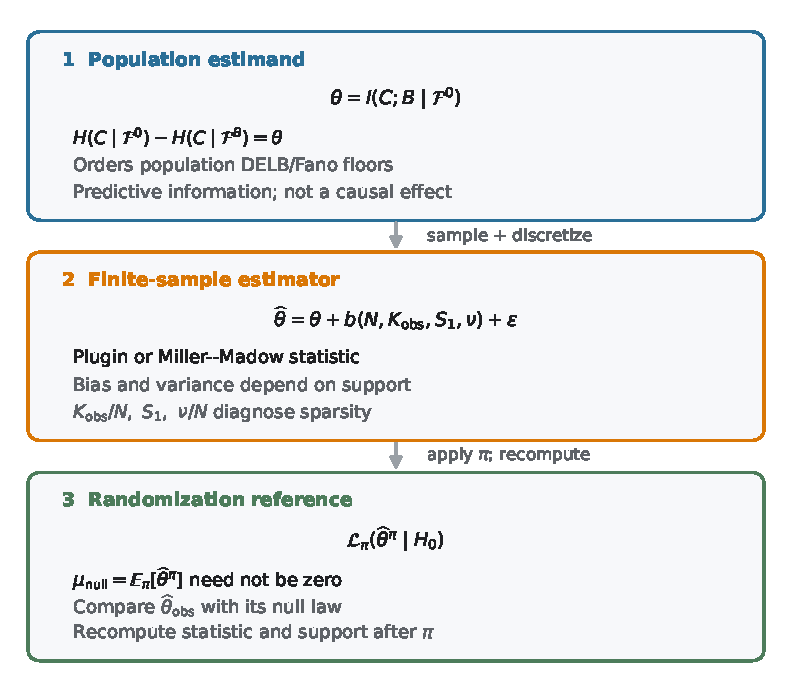
\includegraphics[width=0.92\textwidth]{figures/s7/e15_estimand_estimator_null_wide.pdf}
\caption{Population estimand, finite-sample estimator, and
transformation-specific randomization reference. CMI denotes predictive
information and is not interpreted as a causal effect.}
\label{fig:three_layers}
\end{figure}

\subsubsection{Known-Truth Sparse Nested-State Simulation}
\label{subsec:e12_simulation_methods}

Finite-sample behavior was evaluated under a fully enumerated probability
model. The baseline state \(Z\) had 4, 16, or 64 categories, the added state
\(B\) had 2, 4, or 8 categories, and the integer target followed a
negative-binomial conditional distribution. The factorial design crossed
sample sizes 365 and 1095; balanced and skewed state probabilities; zero,
moderate, and stronger population CMI; and independent or persistent Markov
state sequences. Exact summation, with the truncated tail below the
prespecified tolerance, supplied population CMI rather than treating a
large simulated sample as truth.

For each of 216 estimator cells, 150 samples were generated, yielding
32,400 replicate records. Both plug-in and Miller--Madow CMI were computed
with the same functions used in the empirical analysis, along with
\(K_{\mathrm{obs}}/N\), \(S_1\), and \(\nu/N\). A second experiment applied
the same temporal-block, spatial-series, and circular-shift transformations
to population-null and positive-CMI samples. It comprised 30 Monte Carlo
datasets per cell and 99 transformations per estimator and null design.
The reported Type I rejection rate and power assess those
specific data-generating and transformation mechanisms rather than all CMI
estimators or randomization schemes.

\subsection{DELB-Based Evaluation Algorithm}
\label{subsec:delb_evaluation_algorithm}

\begin{Algorithm}[DELB-based evaluation of an added urban data source]
\label{alg:delb_evaluation}
\textbf{Input:} integer target \(C\); baseline state \(\mathcal S^0\);
added-data state \(B\); training, validation, and test indices; entropy
estimator; randomization designs; number of repetitions \(R\).\\
\textbf{Output:} \(\widehat L^0\), \(\widehat L^B\),
\(\widehat{\Delta L}\), \(\widehat I(C;B\mid\mathcal S^0)\), support
diagnostics, randomization \(p\)-values, and matched held-out prediction
errors.
\begin{enumerate}
    \item Estimate all discretization thresholds from the training period
    and freeze them for validation and testing.
    \item Construct the baseline state \(\mathcal S^0\) and augmented state
    \(\mathcal S^B=(\mathcal S^0,B)\) on identical eligible observations.
    \item Estimate \(\widehat H(C\mid\mathcal S^0)\) and
    \(\widehat H(C\mid\mathcal S^B)\) with the same entropy estimator.
    \item Numerically evaluate
    \(\widehat L^j=\mathcal H_{\mathbb Z}^{-1}
    [\widehat H(C\mid\mathcal S^j)]\), \(j\in\{0,B\}\).
    \item Compute raw CMI, the absolute and relative estimated DELB
    reductions, and the support-density, singleton-share, and effective
    degrees-of-freedom diagnostics.
    \item For each prespecified randomization design and repetition, transform
    \(B\), reconstruct \(\mathcal S^B\), and recompute both state support and
    the complete statistic; then calculate plus-one upper-tail \(p\)-values.
    \item Fit each prediction model twice with matched samples, training
    windows, tuning rules, and all non-bicycle inputs: once with
    \(\mathcal S^0\) and once with \(\mathcal S^B\).
    \item Compare the estimated DELB change, randomization-calibrated evidence,
    and held-out MSE change as three separate outputs.
\end{enumerate}
\end{Algorithm}

\paragraph{Numerical inversion.}
For a positive entropy value, the implementation brackets the
discrete-Gaussian rate \(\lambda\) from an initial value of \(1\) by repeated
halving or doubling and then applies Brent's method. The root tolerance is
\(10^{-12}\), with at most 200 iterations. For \(\lambda\geq1\), the
partition function and second moment are evaluated by direct symmetric
integer-lattice summation. For \(\lambda<1\), the Poisson-dual theta series
avoids an unnecessarily wide real-lattice truncation. In both cases the
support radius is expanded until the analytic bound on the omitted
two-sided unnormalized tail is at most \(10^{-15}\). Entropy values at or
below zero map to a DELB of zero. Repeated resampling and randomization paths
use the configured monotone interpolation grid over 0--8 bits, with direct
inverse evaluations retained for validation.

\paragraph{Computational cost and parallelization.}
Let \(N\) be the number of matched observations, \(K_0\) and \(K_B\) the
numbers of occupied atoms in the two state tables, \(M\) the maximum retained
half-support of a lattice sum, \(T\leq200\) the number of root evaluations,
and \(J\) the number of entropy values converted to bounds. State counting
requires \(O(N)\) time and \(O(K_0+K_B)\) memory; direct bound conversion
requires \(O(JTM)\) time and \(O(M)\) additional memory. With \(R\)
randomizations, the serial calibration cost is
\(O(RN+RJTM)\), excluding model fitting, whose cost depends on the selected
predictor. Randomizations are independent conditional on their stored seeds.
The implementation evaluates city--spatial-scale--temporal-scale cells
independently and records cell-level results and seeds for reproducibility.


\subsection{City and Local DELB Estimation}
\label{subsec:city_local_information}

City-level DELB point estimates were evaluated in both training-period-frozen
populations and separately by year. The complete crime-supported domain
represents the full prespecified target population, whereas the
bicycle-covered domain represents the service-covered population in which
the added mobility channel is observed. Both sets of cells were determined
from 2020--2021 records and then applied unchanged to validation and
testing; no 2022 outcome was used to redefine either spatial population.
Their comparison therefore concerns the target analysis population rather
than an administratively fixed city boundary.

Uncertainty was evaluated with 1000 shared non-overlapping seven-day
calendar-block resamples. Resampling an entire city-day block preserved
contemporaneous dependence among grids. Reported 95\% intervals were
centered bootstrap intervals. The co-primary population designation is
limited to the city-level point-estimate comparison. Local estimation,
randomization calibration, held-out prediction, and multiscale analyses
retain their prespecified bicycle-covered domains because complete-domain
counterparts were not generated for all of those experiments.

The calculation was repeated within each grid after removing the grid
identifier from the local state. Eligibility required 1095 valid lagged
days, at least 30 crimes, at least 55 positive-flow days, no zero-flow run
longer than 365 days, and at least two observed target and bicycle states.
This yielded \TotalEligibleLocalGrids{} eligible cells. A one-sided
normal screen based on the seven-day block bootstrap was adjusted by the
Benjamini--Hochberg procedure \citep{benjamini1995}; because state-space
sparsity can bias entropy differences, it is described as a
\emph{sampling-uncertainty screen}, not as a randomization test of
conditional independence. Spatial clustering was summarized with global
and local Moran statistics \citep{moran1950} using row-standardized queen
contiguity and 999 permutations.

\subsection{Three-Axis Scale and Sample-Size Design}
\label{subsec:e16_scale_methods}

To distinguish changes in the prediction target from changes in estimator
stability, the multiscale design crossed three spatial resolutions (500~m,
1~km, and 2~km),
two temporal resolutions (day and complete ISO week), and five sample
fractions (20, 40, 60, 80, and 100\%). The comparison domain comprised
complete 2~km parents, their four 1~km children, and all sixteen 500~m
descendants. Crime and bicycle totals reconciled exactly across this nested
common footprint. Weekly records were sums over seven complete days, and a
one-period lag always referred to the preceding aggregation period.

Sample fractions were formed by retaining all grids in selected time blocks.
Daily panels used complete seven-day blocks and weekly panels used complete
four-week blocks, stratified by year and season. Fractions were nested within
each of 50 frozen repetitions; a separate five-point expanding-window design
diagnosed chronological accumulation and possible distribution drift.
Estimator stability was measured by
\begin{equation}
S_N(\widehat\theta)
=\frac{|\widehat\theta_N-\widehat\theta_{N_{\max}}|}
{\max(|\widehat\theta_{N_{\max}}|,10^{-12})},
\label{eq:e16_stability}
\end{equation}
where \(\widehat\theta\) denotes an estimated entropy, CMI, or DELB quantity.
It measures convergence to the full-sample estimate, not error relative to
unknown population truth.

Count-level DELBs remained primary. For a square-cell area \(A\) in km\(^2\)
and aggregation duration \(\tau\) in days, the deterministically scaled crime
intensity target has
\begin{equation}
L_{\mathrm{int,MSE}}^{j}(A,\tau)
=\frac{L^{j}(A,\tau)}{(A\tau)^2},
\qquad
L_{\mathrm{int,RMSE}}^{j}(A,\tau)
=\frac{\sqrt{L^{j}(A,\tau)}}{A\tau},
\quad j\in\{0,B\}.
\label{eq:e16_intensity_normalization}
\end{equation}
The transformation applies to the correspondingly scaled count target; it
does not make daily and weekly targets, or different spatial aggregates, the
same estimand. No DELB or CMI was divided by sample size.

Randomization calibration covered all 90 city--space--time--sample cells.
Each cell used 199 temporal-block, spatial-series, and circular-shift
replicates; the prespecified 500~m--day, 1~km--day, and 2~km--week scales used
999 replicates. Fractions below 100\% used the lowest-index frozen thinning
path (replicate 1), whereas the stability analysis separately summarized all
50 thinning paths. Temporal blocks contained seven days or four weeks;
circular shifts were separated by at least 31 days or five weeks.
Miller--Madow CMI, DELB reduction, support atoms, singleton share, and
effective degrees of freedom were recomputed after every transformation.
Plus-one upper-tail \(p\)-values were adjusted both across all 270 tests and
within city--null-design families. These are design-conditioned diagnostics
rather than exact conditional randomization tests.

\subsection{Matched Prediction and Predictability Gap}
\label{subsec:prediction_experiment}
\label{subsec:methods_prediction}

Four model families were compared under the paired states in
Equations~\eqref{eq:empirical_baseline_state} and
\eqref{eq:empirical_bicycle_state}: a smoothed state mean, a Poisson
generalized linear model (GLM), a negative-binomial GLM, and histogram
gradient boosting with Poisson loss. Within each family, baseline and
bicycle-aware specifications used the same target, sample, preprocessing,
training period, tuning rule, and integer post-processing. The bicycle-aware
version added only \(Q_B(B^{\mathrm{total}}_{t-1})\). A seven-day seasonal
naive predictor was retained as an external descriptive benchmark but was
not matched to the DELB state and was not used in the principal comparisons.

Hyperparameters were selected by validation-period integer MSE. Continuous
nonnegative predictions were converted to integer counts using half-up
rounding. The primary metric was
\begin{equation}
\operatorname{MSE}^{j}_{c,k}
=\frac{1}{N_c}\sum_{(i,t)\in\mathcal T_c}
\left(C_{c,i,t}-\widehat C^{\,j}_{c,i,t,k}\right)^2,
\quad j\in\{0,B\},
\label{eq:empirical_mse}
\end{equation}
where \(k\) indexes the model family and \(\mathcal T_c\) is the fixed
July--December 2022 test set. Positive
\(\Delta\operatorname{MSE}_{c,k}
=\operatorname{MSE}^{0}_{c,k}-\operatorname{MSE}^{B}_{c,k}\)
denotes improvement. One thousand shared non-overlapping seven-day test
blocks preserved cross-grid dependence. Family-level screens used
one-sided normal approximations and Benjamini--Hochberg adjustment.

\subsection{Secondary Fano, Heterogeneity, and Robustness Designs}
\label{subsec:fano_validation_methods}

Fixed finite-label targets complemented the integer-count MSE analysis. The
primary target was
\[
Y^{(2)}_{c,i,t}=\mathbf 1\{C_{c,i,t}>0\},
\]
and the robustness target mapped \(C=0\), \(C=1\), and \(C\geq2\) to three
classes. These thresholds were fixed globally and were not selected from
city or test outcomes. Baseline and bicycle-augmented states were exactly those
in Equations~\eqref{eq:empirical_baseline_state} and
\eqref{eq:empirical_bicycle_state}.

Conditional entropy and the Fano floor were estimated on the combined
training and validation period. A statewise modal classifier was then
evaluated on the unchanged July--December 2022 test period. Test states
unseen before July 2022 used the pretest global mode; no test label was used
to set a fallback. Uncertainty used 300 non-overlapping seven-day
calendar-block bootstrap samples. Centered intervals were reported because
unconditional resampling can itself remove rare states; the raw bootstrap
means were retained as diagnostics.

An oracle check reused the enumerated simulation models and compared the
true Bayes error with the true Fano floor for binary and three-level targets.
The empirical comparison contrasted an estimated pretest floor with a held-out
classifier error. Estimated violations, if present, were retained as
finite-sample or distribution-shift diagnostics. DELB and Fano values were
never numerically compared because their targets and losses differ.

\subsubsection{Predictability Gap and Theory--Practice Comparison}
\label{subsec:gap_methods}
\label{subsec:gap_efficiency}

The model-specific predictability gap was
\begin{equation}
G^j_{c,k}=\operatorname{MSE}^{j}_{c,k}-L^j_c
\label{eq:empirical_gap}
\end{equation}
and its narrowing,
\begin{equation}
\Delta G_{c,k}
=G^0_{c,k}-G^B_{c,k}
=\Delta\operatorname{MSE}_{c,k}-\Delta L_c.
\label{eq:empirical_gap_narrowing}
\end{equation}
In population notation, the same accounting quantity is
\begin{equation}
G=\operatorname{MSE}-L,
\label{eq:prediction_gap}
\end{equation}
and an information-use ratio may be reported only when its denominator is
positive:
\begin{equation}
\eta=\frac{\Delta\operatorname{MSE}}{\Delta L}.
\label{eq:bound_efficiency}
\end{equation}
A positive \(\Delta G\) means that empirical error fell by more than the
estimated floor; a negative value means that the theoretical opportunity
expanded faster than the tested model used it. For the test comparison,
the exact bounds were re-estimated on the matched test-window information
states.

At the local scale, pretest \(\Delta L_{c,i}\) from training plus
validation was compared with test-period
\(\Delta\operatorname{MSE}_{c,i,k}\). Spearman correlations used 2000
paired-grid bootstrap resamples and false-discovery-rate adjustment.
Separate ordinary least-squares models regressed local empirical
improvement on local theoretical reduction with city fixed effects and
HC3 standard errors. These analyses are descriptive: cross-grid dependence
was not modeled in the regression covariance.

\subsubsection{Crime-Type Heterogeneity}
\label{subsec:crime_type_methods}

The information and matched-prediction analyses were repeated for property
theft, vehicle theft, and burglary, using category-specific lagged counts
but the same bicycle thresholds and temporal split. This produced 18
city--category theory estimates (pooled and test), 36 paired test prediction
contrasts, and paired within-city category comparisons. Seven-day block
resampling and Benjamini--Hochberg adjustment were applied as in the primary
experiments.

\subsubsection{Alternative Specifications and Null Calibration}
\label{subsec:robustness_null_methods}

Prespecified robustness analyses examined whether the sign of the estimated
DELB reduction persisted across design changes. The 16 theory
specifications comprised
500~m, 1~km, and 2~km grids; daily and weekly targets; alternative crime and
bicycle state mappings; crime and bicycle lags through seven days; and
inflow, outflow, and absolute net flow. Each specification was estimated
with plug-in, Miller--Madow, and a coherent Jeffreys--Dirichlet estimator.
For the latter, a single symmetric Dirichlet posterior was placed on the
observed atoms of \((C_t,\mathcal S^0_t,B_{t-1})\), and both conditional
entropies were obtained by marginal aggregation of that posterior. Bootstrap
intervals were recomputed with 7-, 14-, and 28-day blocks. Predictive
stability was assessed at 12 expanding monthly origins in 2022, each with a
one-month evaluation window and the same four model families.

Three diagnostics assessed whether the observed CMI exceeded finite-sample
reference distributions. A temporal-block permutation reassigned seven-day mobility
blocks, a spatial-series permutation reassigned entire mobility histories
among grids, and a circular-shift surrogate displaced each grid's mobility
series by an admissible random offset. Each design used 999 transformations,
upper-tail randomization \(p\)-values, and Benjamini--Hochberg correction.
The same designs were applied to the 339 eligible grids. A local cell
was declared null-calibrated only if it passed all three adjusted tests.
Finally, matched 14- and 30-day mobility lags were compared with the recent
one-day lag. These procedures are diagnostic randomization tests, not exact
conditional randomization tests and not tests of a causal bicycle effect.

E17 assessed whether the city-level calibration depended on the primary
Miller--Madow correction. On each of the identical E10 surrogates, it
recomputed plug-in, Miller--Madow, and coherent observed-support
Jeffreys--Dirichlet CMI. Plus-one upper-tail \(p\)-values were adjusted in
two prespecified families: nine city--design comparisons within each
estimator and all 27 estimator--city--design comparisons globally. E17 did
not rerun the 339-cell local screen. The Jeffreys calculation regularizes
the probabilities of observed full-joint atoms; it does not impute
unobserved support.

E18 added a baseline-state-matched restricted randomization at the city
level. Each grid series was partitioned into complete seven-day blocks.
Blocks were permuted without replacement within grid, year, and season
after ordering them by the distribution of lagged-crime states and holiday
occupancy; strata with fewer than five blocks were widened within year.
Terminal incomplete blocks remained fixed. The design used 999
randomizations, plus-one upper-tail \(p\)-values, and a three-city
Benjamini--Hochberg family. Prespecified diagnostics required at least 80\%
of blocks to be movable and an absolute standardized difference no larger
than 0.10 for the bicycle-state marginal.

A semi-synthetic experiment evaluated calibration and power on fixed
empirical state supports. Six flow-quantile-spanning grids and 365 days
were selected deterministically per city. Negative-binomial targets were
generated from shrinkage estimates depending only on the baseline state
under the null; centered bicycle-state effects were then calibrated by
enumeration to target population CMI values of 0, 0.02, 0.05, and 0.10
bit, subject to the maximum attainable value on each support. The factorial
design crossed three cities, fitted and enhanced-overdispersion scenarios,
and the original temporal-block and restricted matched-block references.
Each cell used 50 Monte Carlo datasets and 99 randomizations. Exact
binomial 95\% intervals accompanied Type I error and power. This restricted
design is closer to the baseline state than E10, but it is not an exact
conditional randomization test because it does not sample from a known
\(B\mid\mathcal S^0\) distribution.

\subsubsection{Surrogate-Specific Support Diagnostics}
\label{subsec:e13_support_methods}

Each accepted surrogate was reconstructed from its original seed, after which
both CMI and state support were recomputed. For each observed or randomized
sample, the recorded quantities were
\begin{equation}
K_{\mathrm{obs}}
=\#\{(C,Z,B)\text{ observed atoms}\},
\qquad
S_1
=\frac{\#\{\text{observations in singleton atoms}\}}{N},
\label{eq:e13_support_metrics}
\end{equation}
and
\begin{equation}
\nu=\sum_z(r_z-1)(c_z-1),
\label{eq:e13_effective_df}
\end{equation}
where \(r_z\) and \(c_z\) are the observed target and bicycle-state
cardinalities within baseline state \(z\). The analysis used
\(K_{\mathrm{obs}}/N\), \(S_1\), and \(\nu/N\).

Simulation-based associations related null bias to these support
metrics. Empirical associations were reported descriptively with
Spearman correlations and city and null-design fixed-effects regressions
using city-grid-clustered standard errors. Models related the null mean to
mean surrogate support and observed-minus-null CMI to surrogate-minus-
observed support change. These associations diagnose a finite-support
mechanism; they do not turn the null mean into an estimator-bias estimate or
identify a causal effect.

\subsection{Reproducibility and Analysis Scope}
\label{subsec:reproducibility}

Every experiment was executed through a Python entry point configured by a
versioned YAML file. Run directories contain environment
snapshots, random seeds, source-run pointers, row reconciliations, acceptance
checks, machine-readable tables, diagnostic workbooks, and figures. All
manuscript figures were generated by the corresponding Python experiment;
none was manually edited. E11 reads only accepted E02 and E04--E10 outputs,
while the S7 Python synthesis reads accepted E12--E15 outputs and copies a
hash-verified figure set into the manuscript. E09 and E10 were frozen before
output inspection; E12--E14 retain replicate-level simulation, support, and
bootstrap records; E15 retains both single- and double-column vector
versions of the conceptual figure. All accepted outputs remain in the
versioned run lineage. E16 similarly reads only accepted multiscale panels,
sample indices, estimates, and randomization outputs; its S16.7 Python
synthesis generates the LaTeX macros and tables and copies all scale figures
after SHA-256 verification. A minimal known-truth example at
\texttt{examples/minimal\_delb\_cmi\_simulation.py} reproduces the population
CMI ordering and discrete-envelope DELB inversion without city data; it is pedagogical and
does not replace the registered E12 simulation grid.
